\documentclass[11pt]{article}\usepackage[]{graphicx}\usepackage[]{color}
%% maxwidth is the original width if it is less than linewidth
%% otherwise use linewidth (to make sure the graphics do not exceed the margin)
\makeatletter
\def\maxwidth{ %
  \ifdim\Gin@nat@width>\linewidth
    \linewidth
  \else
    \Gin@nat@width
  \fi
}
\makeatother

\definecolor{fgcolor}{rgb}{0.345, 0.345, 0.345}
\newcommand{\hlnum}[1]{\textcolor[rgb]{0.686,0.059,0.569}{#1}}%
\newcommand{\hlstr}[1]{\textcolor[rgb]{0.192,0.494,0.8}{#1}}%
\newcommand{\hlcom}[1]{\textcolor[rgb]{0.678,0.584,0.686}{\textit{#1}}}%
\newcommand{\hlopt}[1]{\textcolor[rgb]{0,0,0}{#1}}%
\newcommand{\hlstd}[1]{\textcolor[rgb]{0.345,0.345,0.345}{#1}}%
\newcommand{\hlkwa}[1]{\textcolor[rgb]{0.161,0.373,0.58}{\textbf{#1}}}%
\newcommand{\hlkwb}[1]{\textcolor[rgb]{0.69,0.353,0.396}{#1}}%
\newcommand{\hlkwc}[1]{\textcolor[rgb]{0.333,0.667,0.333}{#1}}%
\newcommand{\hlkwd}[1]{\textcolor[rgb]{0.737,0.353,0.396}{\textbf{#1}}}%

\usepackage{framed}
\makeatletter
\newenvironment{kframe}{%
 \def\at@end@of@kframe{}%
 \ifinner\ifhmode%
  \def\at@end@of@kframe{\end{minipage}}%
  \begin{minipage}{\columnwidth}%
 \fi\fi%
 \def\FrameCommand##1{\hskip\@totalleftmargin \hskip-\fboxsep
 \colorbox{shadecolor}{##1}\hskip-\fboxsep
     % There is no \\@totalrightmargin, so:
     \hskip-\linewidth \hskip-\@totalleftmargin \hskip\columnwidth}%
 \MakeFramed {\advance\hsize-\width
   \@totalleftmargin\z@ \linewidth\hsize
   \@setminipage}}%
 {\par\unskip\endMakeFramed%
 \at@end@of@kframe}
\makeatother

\definecolor{shadecolor}{rgb}{.97, .97, .97}
\definecolor{messagecolor}{rgb}{0, 0, 0}
\definecolor{warningcolor}{rgb}{1, 0, 1}
\definecolor{errorcolor}{rgb}{1, 0, 0}
\newenvironment{knitrout}{}{} % an empty environment to be redefined in TeX

\usepackage{alltt}
\usepackage{amsmath}
\usepackage{stmaryrd}
\usepackage{bbm}
\usepackage{amsmath}
\usepackage{mathtools}
\usepackage{pdfpages}
\usepackage{breqn}

\newcount\colveccount
\newcommand*\colvec[1]{
        \global\colveccount#1
        \begin{pmatrix}
        \colvecnext
}
\def\colvecnext#1{
        #1
        \global\advance\colveccount-1
        \ifnum\colveccount>0
                \\
                \expandafter\colvecnext
        \else
                \end{pmatrix}
        \fi
}
\newcommand{\argmin}{\arg\!\min}

\author{Thibault Doutre, Student ID 26980469}
\title{STAT230 HW 6 \\
University of California, Berkeley}
\date{\today}
\IfFileExists{upquote.sty}{\usepackage{upquote}}{}
\begin{document}
\maketitle

\section{}
The log likelihood is equal to:
\begin{align}
l(\theta|X) &= log \prod_{i=1}^n \frac{\theta}{(\theta+X_i)^2} \\
&= \sum_{i=1}^n log \frac{\theta}{(\theta+X_i)^2} \\
&= \sum_{i=1}^n log(\theta)-2log(\theta+X_i)\\
&= n \times log(\theta) - 2\sum_{i=1}^n log(\theta+X_i)
\end{align}

\begin{knitrout}
\definecolor{shadecolor}{rgb}{0.969, 0.969, 0.969}\color{fgcolor}\begin{kframe}
\begin{alltt}
\hlcom{## # Load data}
\hlstd{data} \hlkwb{=} \hlkwd{read.table}\hlstd{(}\hlstr{'mle.txt'}\hlstd{)}
\hlstd{data} \hlkwb{=} \hlkwd{unlist}\hlstd{(data,} \hlkwc{use.names} \hlstd{=} \hlnum{FALSE}\hlstd{)}
\hlstd{n} \hlkwb{=} \hlkwd{length}\hlstd{(data)}

\hlcom{## # Compute log likelihood}
\hlstd{log_likelihood_aux} \hlkwb{=} \hlkwa{function}\hlstd{(}\hlkwc{theta}\hlstd{)\{}
  \hlstd{n}\hlopt{*}\hlkwd{log}\hlstd{(theta)} \hlopt{-} \hlnum{2}\hlopt{*}\hlkwd{sum}\hlstd{(}\hlkwd{log}\hlstd{(theta}\hlopt{+}\hlstd{data))}
\hlstd{\}}
\hlstd{log_likelihood} \hlkwb{=} \hlkwd{Vectorize}\hlstd{(log_likelihood_aux)}

\hlcom{# Plot}
\hlstd{thetas} \hlkwb{=} \hlkwd{seq}\hlstd{(}\hlkwc{from} \hlstd{=} \hlnum{0.1}\hlstd{,} \hlkwc{to} \hlstd{=} \hlnum{100}\hlstd{,} \hlkwc{by} \hlstd{=} \hlnum{0.1}\hlstd{)}
\hlstd{lls} \hlkwb{=} \hlkwd{log_likelihood}\hlstd{(thetas)}
\hlkwd{plot}\hlstd{(thetas,lls,}
     \hlkwc{main} \hlstd{=} \hlstr{"Log likelihood of the data"}\hlstd{,}
     \hlkwc{ylab} \hlstd{=} \hlstr{"Log Likelihood"}\hlstd{,}
     \hlkwc{xlab} \hlstd{=} \hlstr{"Theta"}\hlstd{,}
     \hlkwc{type}\hlstd{=}\hlstr{"l"}\hlstd{)}
\end{alltt}
\end{kframe}
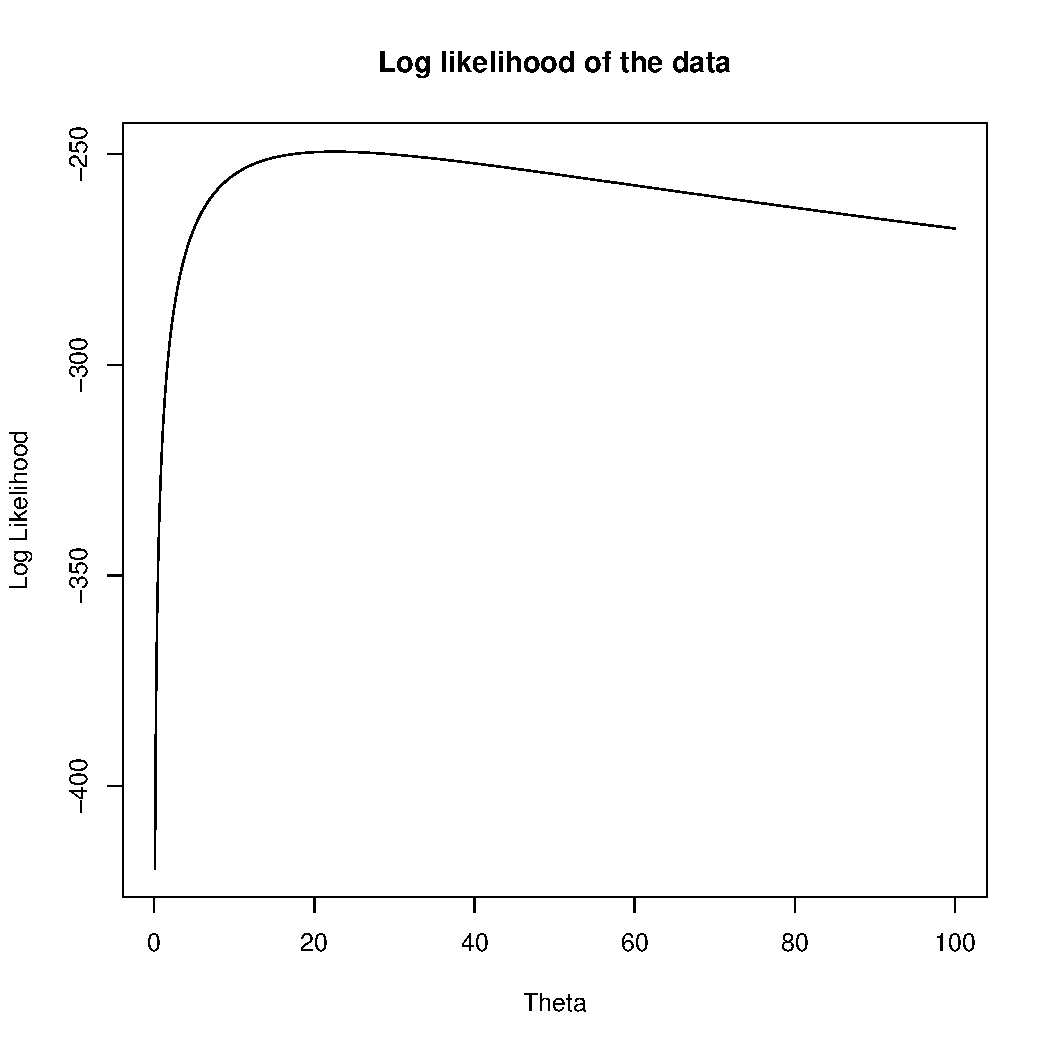
\includegraphics[width=\maxwidth]{figure/unnamed-chunk-1-1} 

\end{knitrout}


\section{}
First, I parametrize again $l$ with $\exp(\phi)=\theta$, so the likelihood is defined on $R$. I obtain:
\begin{align}
l(\phi|X) &= n \phi - 2\sum_{i=1}^n log(\exp(\phi)+X_i)
\end{align}
\begin{knitrout}
\definecolor{shadecolor}{rgb}{0.969, 0.969, 0.969}\color{fgcolor}\begin{kframe}
\begin{alltt}
\hlcom{## # Change variable theta<-exp(phi)}
\hlstd{log_likelihood_phi_aux} \hlkwb{=} \hlkwa{function}\hlstd{(}\hlkwc{phi}\hlstd{)\{}
  \hlstd{n}\hlopt{*}\hlstd{phi} \hlopt{-} \hlnum{2}\hlopt{*}\hlkwd{sum}\hlstd{(}\hlkwd{log}\hlstd{(}\hlkwd{exp}\hlstd{(phi)}\hlopt{+}\hlstd{data))}
\hlstd{\}}
\hlstd{log_likelihood_phi} \hlkwb{=} \hlkwd{Vectorize}\hlstd{(log_likelihood_phi_aux)}

\hlcom{# Plot}
\hlstd{phis} \hlkwb{=} \hlkwd{seq}\hlstd{(}\hlkwc{from} \hlstd{=} \hlopt{-}\hlnum{10}\hlstd{,} \hlkwc{to} \hlstd{=} \hlnum{10}\hlstd{,} \hlkwc{by} \hlstd{=} \hlnum{0.1}\hlstd{)}
\hlstd{lls} \hlkwb{=} \hlkwd{log_likelihood_phi}\hlstd{(phis)}
\hlkwd{plot}\hlstd{(phis,lls,}
     \hlkwc{main} \hlstd{=} \hlstr{"Log likelihood of the data"}\hlstd{,}
     \hlkwc{ylab} \hlstd{=} \hlstr{"Log Likelihood"}\hlstd{,}
     \hlkwc{xlab} \hlstd{=} \hlstr{"Phi"}\hlstd{,}
     \hlkwc{type}\hlstd{=}\hlstr{"l"}\hlstd{)}
\end{alltt}
\end{kframe}
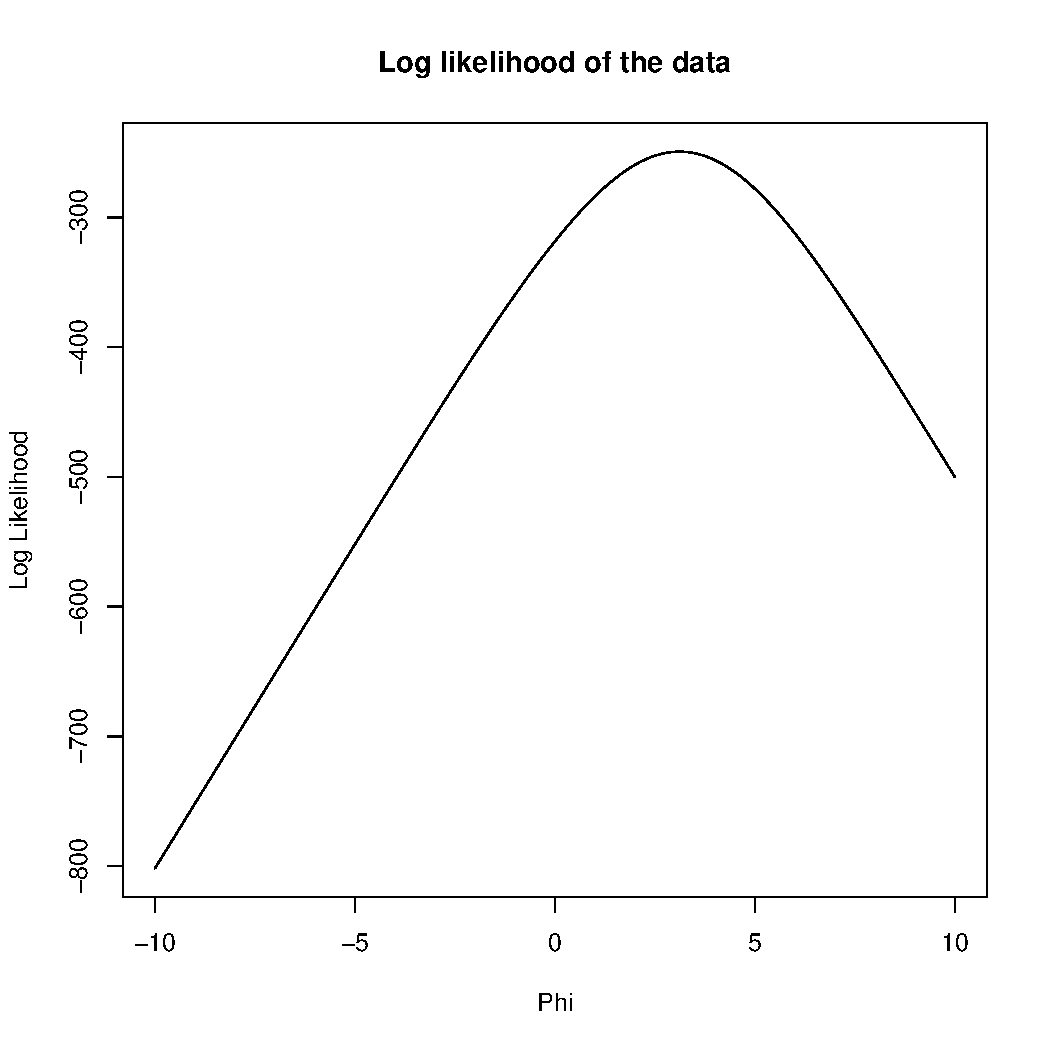
\includegraphics[width=\maxwidth]{figure/unnamed-chunk-2-1} 

\end{knitrout}

Then, I define my function to minimize, to be the opposite of the likelihood.
\begin{knitrout}
\definecolor{shadecolor}{rgb}{0.969, 0.969, 0.969}\color{fgcolor}\begin{kframe}
\begin{alltt}
\hlcom{# Function to optimize}
\hlstd{f} \hlkwb{=} \hlkwa{function}\hlstd{(}\hlkwc{phi}\hlstd{)\{}
  \hlopt{-}\hlkwd{log_likelihood_phi_aux}\hlstd{(phi)}
\hlstd{\}}
\end{alltt}
\end{kframe}
\end{knitrout}
Now, I can find the optimum with the optim function:
\begin{knitrout}
\definecolor{shadecolor}{rgb}{0.969, 0.969, 0.969}\color{fgcolor}\begin{kframe}
\begin{alltt}
\hlstd{opt} \hlkwb{=} \hlkwd{optim}\hlstd{(}\hlnum{0}\hlstd{,f,}
            \hlkwc{method}\hlstd{=}\hlstr{"Brent"}\hlstd{,}
            \hlkwc{lower} \hlstd{=} \hlnum{0}\hlstd{,}
            \hlkwc{upper} \hlstd{=} \hlnum{10}\hlstd{)}
\hlstd{opt}
\end{alltt}
\begin{verbatim}
## $par
## [1] 3.113949
## 
## $value
## [1] 249.3968
## 
## $counts
## function gradient 
##       NA       NA 
## 
## $convergence
## [1] 0
## 
## $message
## NULL
\end{verbatim}
\begin{alltt}
\hlcom{# Plot}
\hlkwd{plot}\hlstd{(phis,lls,}
     \hlkwc{main} \hlstd{=} \hlstr{"Log likelihood of the data"}\hlstd{,}
     \hlkwc{ylab} \hlstd{=} \hlstr{"Log Likelihood"}\hlstd{,}
     \hlkwc{xlab} \hlstd{=} \hlstr{"Phi"}\hlstd{,}
     \hlkwc{type}\hlstd{=}\hlstr{"l"}\hlstd{)}
\hlkwd{points}\hlstd{(opt}\hlopt{$}\hlstd{par,}
       \hlopt{-}\hlstd{opt}\hlopt{$}\hlstd{value,}
       \hlkwc{col} \hlstd{=} \hlstr{"red"}\hlstd{)}
\end{alltt}
\end{kframe}
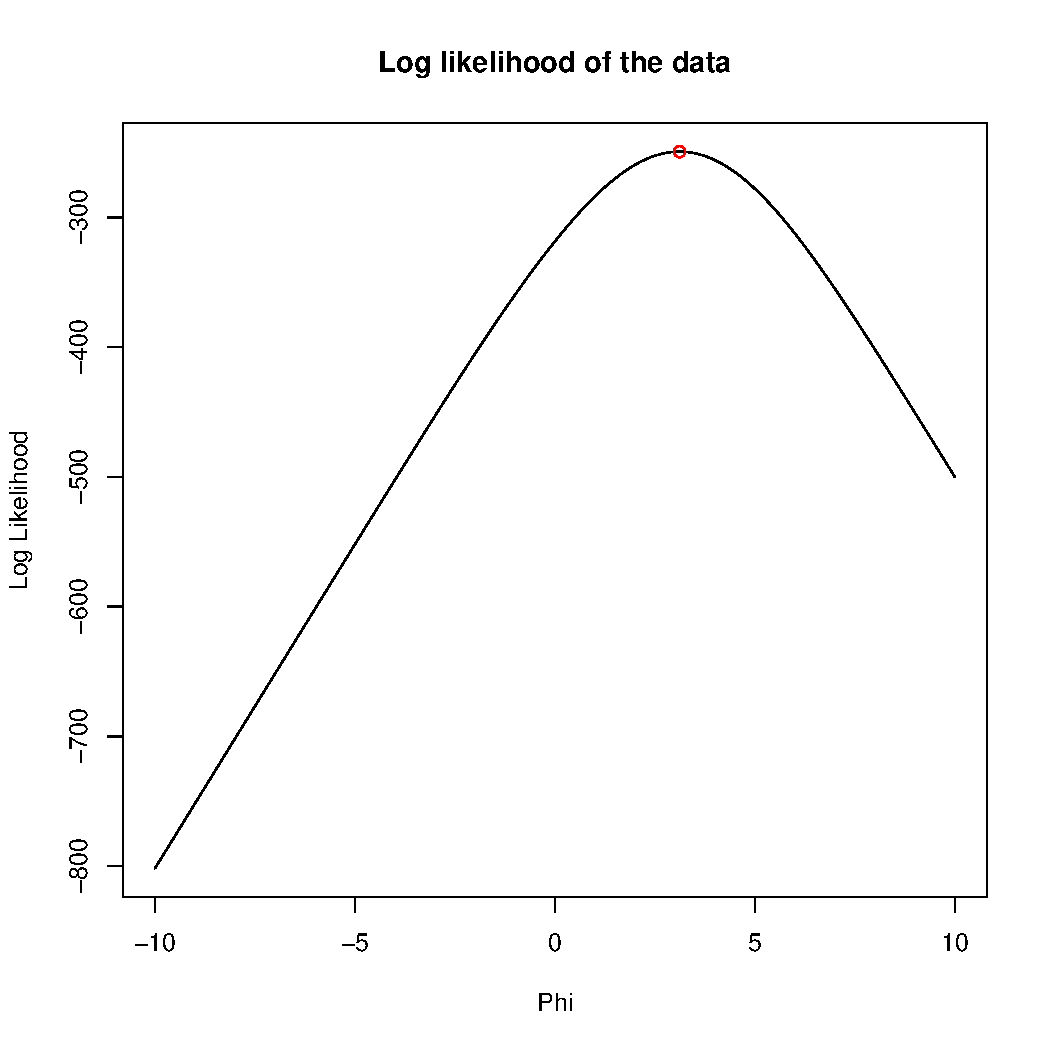
\includegraphics[width=\maxwidth]{figure/unnamed-chunk-4-1} 

\end{knitrout}

\section{}
In order to optimize the log likelihood we can also compute the first two derivatives of the likelihood, and compute the Newton Raphson algorithm. I have coded it by hand:
The first two derivatives are equal to:
\begin{align}
\frac{\partial l(\phi|X)}{\partial \phi} &= n  - 2\sum_{i=1}^n \frac{1}{1+X_i\exp(-\phi)}\\
\frac{\partial^2 l(\phi|X)}{\partial \phi^2} &= -2\exp(-\phi)\sum_{i=1}^n \frac{X_i}{(1+X_i\exp(-\phi))^2}
\end{align}
\begin{knitrout}
\definecolor{shadecolor}{rgb}{0.969, 0.969, 0.969}\color{fgcolor}\begin{kframe}
\begin{alltt}
\hlcom{## # Optimization using derivatives}

\hlcom{# # Compute first derivative}
\hlstd{D_f} \hlkwb{=} \hlkwa{function}\hlstd{(}\hlkwc{phi}\hlstd{)\{}
  \hlopt{-}\hlstd{n} \hlopt{+} \hlnum{2}\hlopt{*}\hlkwd{sum}\hlstd{(}\hlnum{1}\hlopt{/}\hlstd{(}\hlkwd{exp}\hlstd{(}\hlopt{-}\hlstd{phi)}\hlopt{*}\hlstd{data}\hlopt{+}\hlnum{1}\hlstd{))}
\hlstd{\}}
\hlcom{# # Compute second derivative}
\hlstd{D2_f} \hlkwb{=} \hlkwa{function}\hlstd{(}\hlkwc{phi}\hlstd{)\{}
  \hlopt{+} \hlnum{2}\hlopt{*}\hlkwd{exp}\hlstd{(}\hlopt{-}\hlstd{phi)}\hlopt{*}\hlkwd{sum}\hlstd{(data}\hlopt{/}\hlstd{(}\hlkwd{exp}\hlstd{(}\hlopt{-}\hlstd{phi)}\hlopt{*}\hlstd{data}\hlopt{+}\hlnum{1}\hlstd{)}\hlopt{^}\hlnum{2}\hlstd{)}
\hlstd{\}}

\hlcom{# # Newton raphson: one variable}
\hlstd{newton_raphson} \hlkwb{=} \hlkwa{function}\hlstd{(}\hlkwc{start}\hlstd{,}\hlkwc{f}\hlstd{,}\hlkwc{Df}\hlstd{,}\hlkwc{D2f}\hlstd{,}\hlkwc{eps}\hlstd{)\{}
  \hlstd{x_old}\hlkwb{=}\hlstd{start}\hlopt{-}\hlnum{2}\hlopt{*}\hlstd{eps}
  \hlstd{x_new}\hlkwb{=}\hlstd{start}
  \hlkwa{while} \hlstd{(}\hlkwd{abs}\hlstd{(x_new}\hlopt{-}\hlstd{x_old)}\hlopt{>}\hlstd{eps)\{}
    \hlstd{x_old} \hlkwb{=} \hlstd{x_new}
    \hlstd{x_new} \hlkwb{=} \hlstd{x_old} \hlopt{-} \hlkwd{Df}\hlstd{(x_old)}\hlopt{/}\hlkwd{D2f}\hlstd{(x_old)}
  \hlstd{\}}
  \hlkwd{return}\hlstd{(}\hlkwd{list}\hlstd{(}\hlkwc{par} \hlstd{= x_new,} \hlkwc{value} \hlstd{=} \hlkwd{f}\hlstd{(x_new)))}
\hlstd{\}}

\hlstd{eps}\hlkwb{=}\hlnum{10e-5}
\hlstd{nr} \hlkwb{=} \hlkwd{newton_raphson}\hlstd{(}\hlnum{0}\hlstd{,f,D_f,D2_f,eps)}
\hlstd{nr}
\end{alltt}
\begin{verbatim}
## $par
## [1] 3.113949
## 
## $value
## [1] 249.3968
\end{verbatim}
\begin{alltt}
\hlcom{# Plot}
\hlkwd{plot}\hlstd{(phis,lls,}
     \hlkwc{main} \hlstd{=} \hlstr{"Log likelihood of the data"}\hlstd{,}
     \hlkwc{ylab} \hlstd{=} \hlstr{"Log Likelihood"}\hlstd{,}
     \hlkwc{xlab} \hlstd{=} \hlstr{"Phi"}\hlstd{,}
     \hlkwc{type}\hlstd{=}\hlstr{"l"}\hlstd{)}

\hlkwd{points}\hlstd{(nr}\hlopt{$}\hlstd{par,}
       \hlopt{-}\hlstd{nr}\hlopt{$}\hlstd{value,}
       \hlkwc{col} \hlstd{=} \hlstr{"green"}\hlstd{)}
\end{alltt}
\end{kframe}
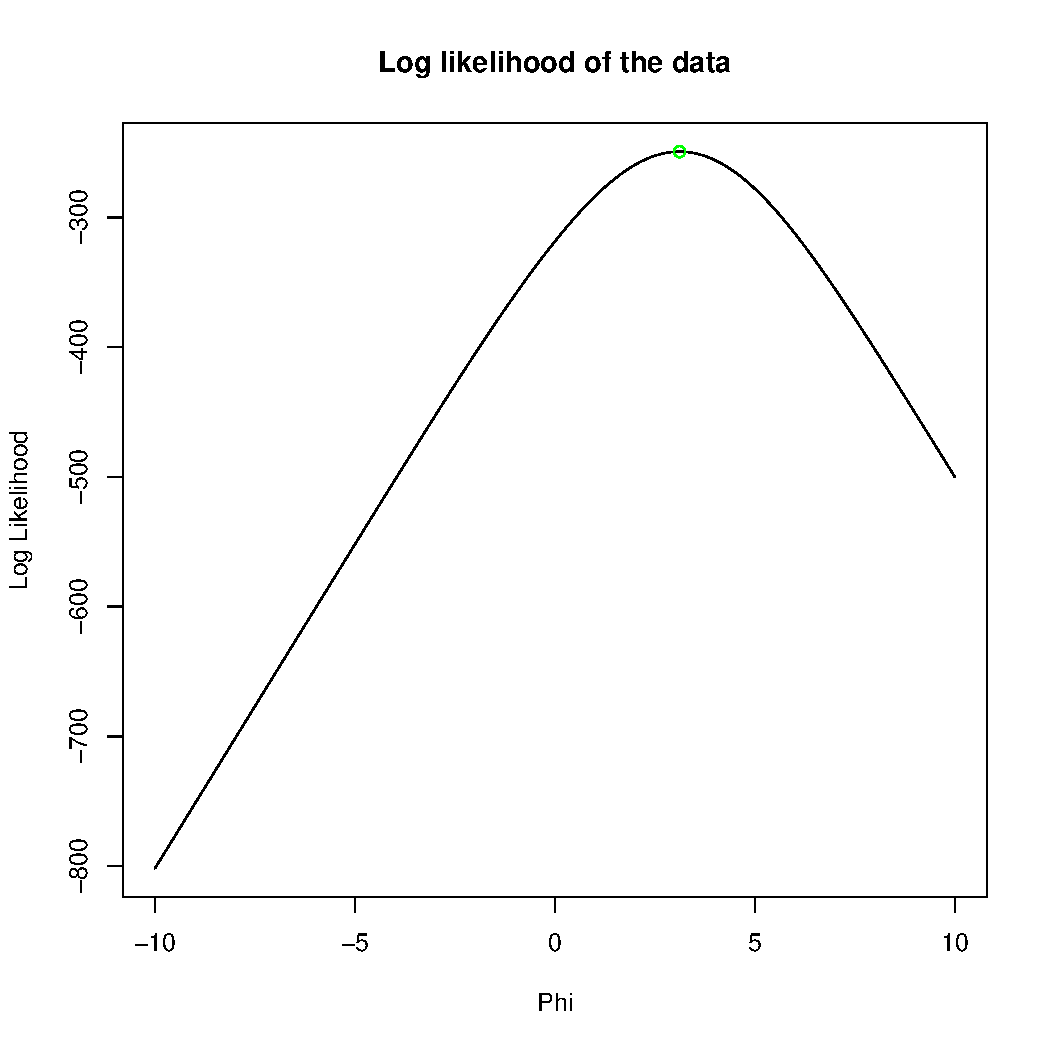
\includegraphics[width=\maxwidth]{figure/unnamed-chunk-5-1} 

\end{knitrout}
The estimated value of theta is then:
\begin{knitrout}
\definecolor{shadecolor}{rgb}{0.969, 0.969, 0.969}\color{fgcolor}\begin{kframe}
\begin{alltt}
\hlstd{theta_hat} \hlkwb{=} \hlkwd{exp}\hlstd{(nr}\hlopt{$}\hlstd{par)}
\hlstd{theta_hat}
\end{alltt}
\begin{verbatim}
## [1] 22.50976
\end{verbatim}
\end{kframe}
\end{knitrout}

\section{}
In order to compute the standard error of $\hat{\theta}$, I use the fact that the asymptotic variance can be computed as $var(\hat{\theta}) = -(\frac{\partial^2 l(\theta|X)}{\partial \theta^2})^{-1}$, where:
\begin{equation}
\frac{\partial^2 l(\theta|X)}{\partial \theta^2} = -\frac{n}{\theta^2}+2\sum_{i=1}^n\frac{1}{(\theta+X_i)^2}
\end{equation}
Then, the SE can be computed as: $SE(\hat{\theta}) = (var(\hat{\theta}))^{1/2}$
\begin{knitrout}
\definecolor{shadecolor}{rgb}{0.969, 0.969, 0.969}\color{fgcolor}\begin{kframe}
\begin{alltt}
\hlcom{## # Standar error on theta}

\hlstd{D2_log_likelihood_theta} \hlkwb{=} \hlkwa{function}\hlstd{(}\hlkwc{theta}\hlstd{)\{}
  \hlopt{-}\hlstd{n}\hlopt{/}\hlstd{theta}\hlopt{^}\hlnum{2}\hlopt{+}\hlnum{2}\hlopt{*}\hlkwd{sum}\hlstd{(}\hlnum{1}\hlopt{/}\hlstd{(theta}\hlopt{+}\hlstd{data)}\hlopt{^}\hlnum{2}\hlstd{)}
\hlstd{\}}

\hlcom{# # Variance}
\hlstd{var_hat} \hlkwb{=} \hlopt{-}\hlnum{1}\hlopt{/}\hlkwd{D2_log_likelihood_theta}\hlstd{(theta_hat)}
\hlcom{# # Standard Error}
\hlstd{se_hat} \hlkwb{=} \hlkwd{sqrt}\hlstd{(var_hat)}
\hlstd{se_hat}
\end{alltt}
\begin{verbatim}
## [1] 5.488464
\end{verbatim}
\end{kframe}
\end{knitrout}



\end{document}









